\documentclass[aspectratio=169]{beamer}

\usepackage[utf8]{inputenc}
\usepackage[T1]{fontenc}
\usepackage[spanish]{babel}
\usepackage{lmodern}
\usepackage{amsmath,amssymb}
\usepackage{graphicx}
\usepackage{booktabs}
\usepackage{array}
\usepackage{tikz}
\usetikzlibrary{babel,arrows.meta,positioning}
\usepackage{listings}
\graphicspath{{figs/}}

\usetheme{Madrid}
\usecolortheme{seahorse}
\setbeamertemplate{navigation symbols}{}
\setbeamerfont{frametitle}{size=\large}

\title[Gas 3D con LGA híbrido]{Expansión de un gas 3D con autómata celular\\y paralelismo híbrido BSPlib + OpenMP}
\subtitle{Propuesta de proyecto --- Laboratorio 2}
\author[Ahumada, Muñoz]{Gonzalo Ahumada \and Daniel Muñoz}
\institute[USACH]{Laboratorio 2 --- High Performance Computing\\[1mm]
           Universidad de Santiago de Chile}
\date{\today}

\begin{document}

\begin{frame}
  \titlepage
\end{frame}

\begin{frame}{Alcance y contenido}
  \begin{block}{Qué es esta presentación}
    \footnotesize
    Describe el \alert{problema}, el \alert{modelo}, la \alert{estrategia de
    paralelización} y el \alert{plan de validación}. Los resultados
    experimentales se reservan para el informe; acá interesa justificar las
    decisiones para poder corregirlas después de la presentación.
  \end{block}
  \tableofcontents
\end{frame}

% ---------------------------------------------------------------------------
\section{Problema y objetivos}
% ---------------------------------------------------------------------------

\begin{frame}{Problema}
  \begin{itemize}
    \item Simular la \alert{expansión de un gas en 3D} sobre una malla cúbica.
    \item Usar un \alert{autómata celular} con reglas locales y estado finito.
    \item Mostrar \alert{paralelismo híbrido}: procesos (BSPlib) + hilos
          (OpenMP).
    \item Requisitos del curso:
      \begin{itemize}
        \item C++, BSPlib para procesos y OpenMP para hilos,
        \item ejecución exigente pero posible en un PC,
        \item objetivo de referencia $4$ procesos $\times$ $8$ hilos,
        \item entregables: código, informe y presentación.
      \end{itemize}
    \item Desafío: comunicación regular, conservación exacta y \emph{scaling}
          en una carga \emph{memory-bound}.
  \end{itemize}
\end{frame}

\begin{frame}{Objetivos}
  \begin{block}{Objetivo general}
    Diseñar e implementar una simulación 3D de expansión de gas con un
    autómata celular y paralelismo híbrido, validada y medible.
  \end{block}
  \begin{block}{Objetivos específicos}
    \footnotesize
    \begin{enumerate}
      \item Definir reglas de CA que conserven masa y momento.
      \item Descomponer el dominio 1D con halos e intercambio BSP.
      \item Paralelizar el cómputo local con OpenMP.
      \item Validar contra la versión serial y medir \emph{scaling}.
      \item Mapear a un gas concreto (neón) para magnitudes físicas.
      \item Documentar decisiones, riesgos y alternativas.
    \end{enumerate}
  \end{block}
\end{frame}

% ---------------------------------------------------------------------------
\section{Modelo físico}
% ---------------------------------------------------------------------------

\begin{frame}{Gas ideal: supuestos y justificación}
  \begin{columns}[T]
    \begin{column}{0.53\textwidth}
      \begin{itemize}
        \item Partículas puntuales, sin fuerzas de largo alcance.
        \item Colisiones binarias elásticas y caos molecular.
        \item Gas noble monoatómico: capa cerrada, $\gamma=5/3$, sin modos
              internos.
        \item A 1 atm y 300 K:
              $Z=1+B_2 n\approx 1.00046$; corrección del \alert{0.05\%}.
      \end{itemize}
    \end{column}
    \begin{column}{0.45\textwidth}
      \begin{block}{Decisión}
        \footnotesize
        Se modela como \alert{gas ideal}. Se desprecian las interacciones
        intermoleculares: en un gas noble a 1 atm son muy débiles y la
        corrección del virial es despreciable.
      \end{block}
      \begin{alertblock}{Limitación declarada}
        \footnotesize
        El autómata es \alert{isotérmico}: no captura el enfriamiento
        adiabático. Se justifica porque el foco es HPC y morfología.
      \end{alertblock}
    \end{column}
  \end{columns}
\end{frame}

\begin{frame}{Elección del gas y mapeo de unidades}
  \begin{columns}[T]
    \begin{column}{0.48\textwidth}
      \centering
      \scriptsize
      \begin{tabular}{lrr}
        \toprule
        & Neón & Helio \\
        \midrule
        $m$ [kg] & $3.35\times10^{-26}$ & $6.65\times10^{-27}$ \\
        $c_{s,\text{iso}}$ [m/s] & 351.6 & 789.4 \\
        $c_{s,\text{ad}}$ [m/s] & 453.9 & 1019.1 \\
        $\rho$ a 1 atm [kg/m$^3$] & 0.8197 & 0.1626 \\
        \bottomrule
      \end{tabular}
      \vspace{2mm}
      \begin{block}{Decisión}
        \scriptsize
        \alert{Neón} por defecto: monoatómico, $c_s$ moderada y densidad fácil
        de verificar. Helio queda como alternativa.
      \end{block}
    \end{column}
    \begin{column}{0.50\textwidth}
      \begin{block}{Mapeo}
        \footnotesize
        \[
          p=\frac{\rho}{3},\qquad c_s^2=\frac{1}{3}
        \]
        \[
          \Delta t=\frac{1}{\sqrt{3}}\frac{\Delta x}{c_{s,\text{iso}}},\qquad
          p\,[\text{Pa}]=\frac{\rho}{3}p_0
        \]
        Con $\Delta x=1$ mm: $\Delta t=1.642\,\mu$s y
        $N_c\approx 8.15\times10^{15}$ moléculas/partícula.
      \end{block}
    \end{column}
  \end{columns}
\end{frame}

% ---------------------------------------------------------------------------
\section{Autómata celular}
% ---------------------------------------------------------------------------

\begin{frame}{Estado del autómata}
  \begin{columns}[T]
    \begin{column}{0.52\textwidth}
      \begin{itemize}
        \item Malla $N\times N\times N$.
        \item 6 bits por celda: $\pm x,\pm y,\pm z$.
        \item Exclusión: máximo una partícula por dirección.
        \item 64 estados posibles (\texttt{uint8\_t}).
        \item Estado entero $\Rightarrow$ conservación exacta.
      \end{itemize}
      \begin{block}{Decisión}
        \footnotesize
        6 direcciones, \alert{sin partícula en reposo}: modelo 3D mínimo,
        1 byte por celda y suficiente para una expansión cualitativa.
      \end{block}
    \end{column}
    \begin{column}{0.44\textwidth}
      \centering
      \begin{tikzpicture}[>=Stealth,font=\small,scale=0.9]
        \node[draw,circle,fill=blue!10,minimum size=8mm] (c) at (0,0) {celda};
        \draw[->,thick] (c) -- (1.1,0)  node[right] {$+x$};
        \draw[->,thick] (c) -- (-1.1,0) node[left]  {$-x$};
        \draw[->,thick] (c) -- (0,1.1)  node[above] {$+y$};
        \draw[->,thick] (c) -- (0,-1.1) node[below] {$-y$};
      \end{tikzpicture}
      \vspace{2mm}
      {\scriptsize $\pm z$: fuera del plano}
    \end{column}
  \end{columns}
\end{frame}

\begin{frame}{Reglas: colisión y streaming}
  \begin{block}{Colisión}
    \footnotesize
    Agrupar estados por $(M,P_x,P_y,P_z)$ y mapear cada uno a otro del mismo
    grupo:
    \[
      M(s')=M(s),\qquad \vec{P}(s')=\vec{P}(s).
    \]
    8 tablas elegidas por celda con un hash global.
  \end{block}
  \begin{block}{Streaming}
    \footnotesize
    Cada bit se mueve a la celda vecina. Formulación \emph{gather}:
    \[
      s^{t+1}_{x,y,z}=(s^t_{x-1,y,z}\wedge B_{+x})
      \vee(s^t_{x+1,y,z}\wedge B_{-x})\vee\cdots
    \]
  \end{block}
  \begin{alertblock}{Invariantes}
    \footnotesize
    Masa y momento total se conservan \alert{exactamente}.
  \end{alertblock}
\end{frame}

\begin{frame}{Justificación del CA y alternativas}
  \centering
  \scriptsize
  \begin{tabular}{>{\raggedright\arraybackslash}p{2.6cm}>{\raggedright\arraybackslash}p{3.5cm}>{\raggedright\arraybackslash}p{3.8cm}>{\raggedright\arraybackslash}p{3.2cm}}
    \toprule
    Modelo & Ventaja & Limitación & Decisión \\
    \midrule
    LGA 6 direcciones & CA estricto, entero, conservativo, 1 byte/celda &
    anisotropía cúbica, isotérmico & \alert{elegido} \\
    LBM D3Q7 & más estable y realista & no es CA estricto, flotantes &
    alternativa \\
    Stencil de densidad & simple y rápido & no es un CA &
    descartado \\
    \bottomrule
  \end{tabular}
  \vspace{3mm}
  \begin{block}{Por qué LGA}
    \footnotesize
    El curso pide \alert{reglas de autómata celular}; el LGA las cumple sin
    ambigüedad. La conservación exacta de masa y momento permite validar el
    paralelismo sin errores de redondeo.
  \end{block}
\end{frame}

% ---------------------------------------------------------------------------
\section{Condiciones iniciales}
% ---------------------------------------------------------------------------

\begin{frame}{Geometrías iniciales}
  \begin{columns}[T]
    \begin{column}{0.48\textwidth}
      \begin{block}{Esfera densa}
        \footnotesize
        \begin{itemize}
          \item $R=\max(6,N/8)$.
          \item $\rho_H=3$ adentro, $\rho_L=0$ afuera.
          \item Cada dirección con $p=1/2$.
          \item Caso base para comparar.
        \end{itemize}
      \end{block}
    \end{column}
    \begin{column}{0.48\textwidth}
      \begin{block}{Cámara de dos presiones}
        \footnotesize
        \begin{itemize}
          \item $\rho_H=3$ ($p_H=1$ atm) para $x<0.25N$.
          \item $\rho_L=0.3$ ($p_L=0.1$ atm) para $x\ge 0.25N$.
          \item Razón $10{:}1$ y rampa de ancho $w$ (\texttt{RAMP}).
          \item Gradiente explícito y medible.
        \end{itemize}
      \end{block}
    \end{column}
  \end{columns}
  \vspace{4mm}
  \begin{block}{Decisión}
    \footnotesize
    Se implementan \alert{ambas}: la esfera como caso base y la cámara para
    estudiar un gradiente de presión controlado. La cámara es la geometría
    principal del experimento.
  \end{block}
\end{frame}

\begin{frame}{Cámara 10:1: parámetros del gradiente}
  \begin{columns}[T]
    \begin{column}{0.50\textwidth}
      \centering
      \begin{tikzpicture}[font=\scriptsize,scale=0.95]
        \draw[->] (0,0) -- (6.4,0) node[right] {$x$};
        \draw[->] (0,0) -- (0,2.5) node[above] {$\rho$};
        \draw[thick] (0,2) -- (1.9,2) -- (2.8,0.4) -- (6.2,0.4);
        \draw[dashed] (1.9,0) -- (1.9,2);
        \draw[dashed] (2.8,0) -- (2.8,0.4);
        \node at (0.8,2.2) {$\rho_H$};
        \node at (5.5,0.65) {$\rho_L$};
        \node at (2.35,1.2) {rampa};
        \node at (1.9,-0.25) {$x_i$};
      \end{tikzpicture}
    \end{column}
    \begin{column}{0.48\textwidth}
      \begin{block}{Valores}
        \footnotesize
        \begin{itemize}
          \item $p_H=1$ atm, $p_L=0.1$ atm.
          \item $x_i=0.25N$, $w=8$ celdas.
          \item $|\nabla p|\approx 0.1125$ atm/mm.
        \end{itemize}
      \end{block}
      \begin{block}{Por qué}
        \footnotesize
        Da una razón de presiones finita, una interfaz clara y una onda de
        expansión medible. Permite comparar con la teoría cualitativa.
      \end{block}
    \end{column}
  \end{columns}
\end{frame}

% ---------------------------------------------------------------------------
\section{Paralelización híbrida}
% ---------------------------------------------------------------------------

\begin{frame}{Modelo BSP: superpasos}
  \centering
  \begin{tikzpicture}[node distance=0.6cm,font=\small,>=Stealth]
    \node[draw,rounded corners,fill=blue!10,align=center] (c)
      {cómputo local\\OpenMP};
    \node[draw,rounded corners,fill=orange!15,right=of c,align=center] (p)
      {\texttt{bsp\_put}\\halos};
    \node[draw,rounded corners,fill=red!10,right=of p,align=center] (s)
      {\texttt{bsp\_sync}\\barrera};
    \node[draw,rounded corners,fill=blue!10,right=of s,align=center] (n)
      {siguiente\\superpaso};
    \draw[->] (c)--(p);
    \draw[->] (p)--(s);
    \draw[->] (s)--(n);
  \end{tikzpicture}
  \vspace{3mm}
  \begin{itemize}
    \item BSPlib sobre MPI (BSPonMPI): $P$ procesos SPMD.
    \item Comunicación \alert{diferida}: se materializa en \texttt{bsp\_sync}.
    \item Costo: $T=\max_i w_i+\max_i h_i g+l$.
  \end{itemize}
  \begin{block}{Decisión}
    \footnotesize
    BSP/BSPlib es requisito del curso y encaja con un stencil regular:
    comunicación por bloques y barrera por superpaso.
  \end{block}
\end{frame}

\begin{frame}{Descomposición de dominio}
  \centering
  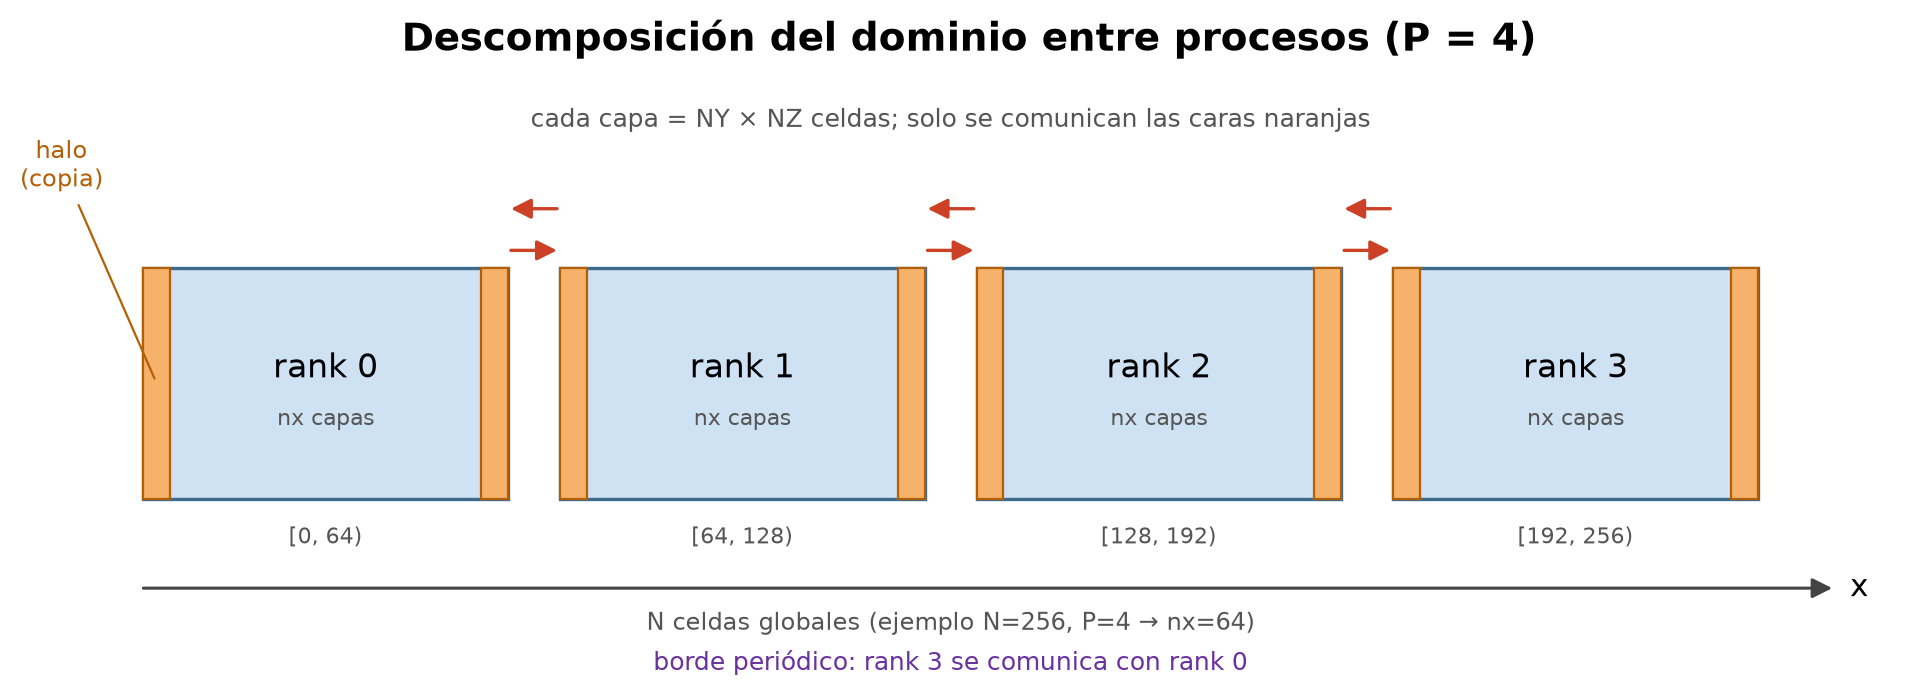
\includegraphics[width=0.98\textwidth]{decomposition.png}\par
  \vspace{-1mm}
  {\scriptsize 1D en $x$; $N$ no necesita ser divisible por $P$. Halos en $x$
   y copias locales en $y,z$.}
\end{frame}

\begin{frame}{Caso $N$ no divisible por $P$}
  \centering
  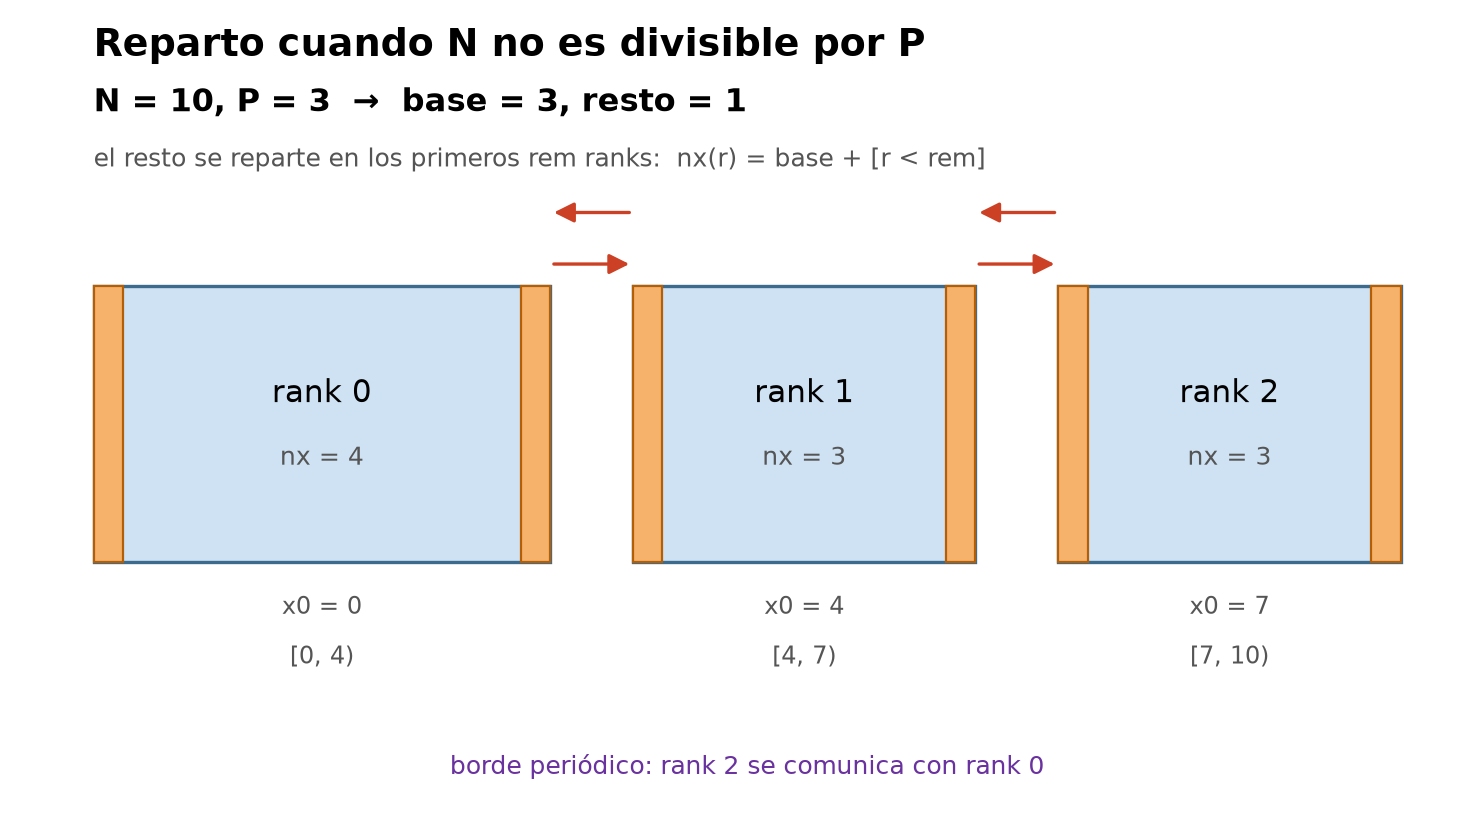
\includegraphics[width=0.82\textwidth]{decomposition_uneven.png}\par
  \vspace{-2mm}
  {\scriptsize $N=10$, $P=3$: rank 0 recibe 4 capas; ranks 1--2 reciben 3.
   Vecinos: $0\leftrightarrow2,1$; $1\leftrightarrow0,2$;
   $2\leftrightarrow1,0$.}
\end{frame}

\begin{frame}{Qué se comunica en cada paso}
  \centering
  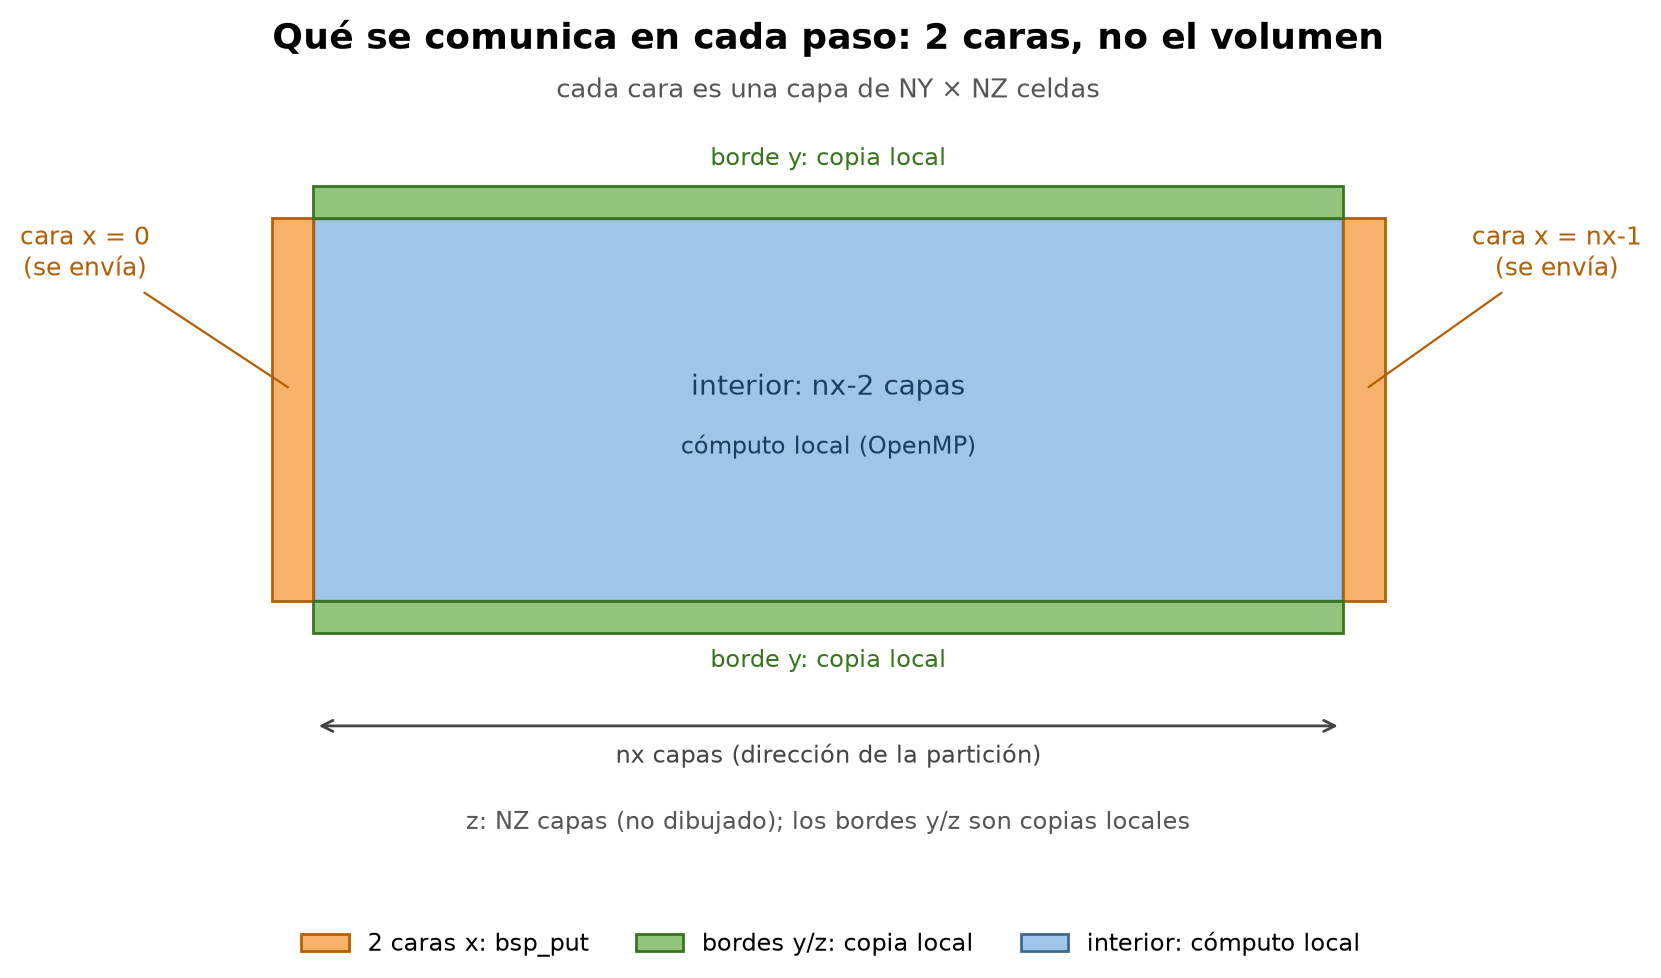
\includegraphics[width=0.80\textwidth]{communication_volume.png}\par
  \vspace{-2mm}
  {\scriptsize Solo las dos caras en $x$; $y,z$ son copias locales.}
\end{frame}

\begin{frame}{Volumen de comunicación por superpaso}
  \begin{block}{Fórmula}
    \[
      V_{\text{rank}} = 2\,(N+2)^2\ \text{bytes},\qquad
      V_{\text{total}} = 2P\,(N+2)^2
    \]
  \end{block}
  \begin{columns}[T]
    \begin{column}{0.48\textwidth}
      \begin{block}{Ejemplo $N=256$, $P=4$}
        \scriptsize
        \begin{tabular}{lr}
          \toprule
          payload por mensaje & 66.6 KB \\
          mensajes por rank/paso & 2 \\
          bytes por rank/paso & 133 KB \\
          bytes totales/paso & 0.53 MB \\
          1000 pasos & 0.53 GB \\
          \bottomrule
        \end{tabular}
      \end{block}
    \end{column}
    \begin{column}{0.48\textwidth}
      \begin{block}{Interpretación}
        \scriptsize
        El volumen local por rank es $n_x N^2 \approx 4.2$ MB. La comunicación
        es $\approx 3\%$ de ese volumen por paso; el costo dominante es la
        barrera y el alltoall de BSPonMPI, no el ancho de banda.
      \end{block}
    \end{column}
  \end{columns}
\end{frame}

\begin{frame}{Vista 3D del subdominio local}
  \centering
  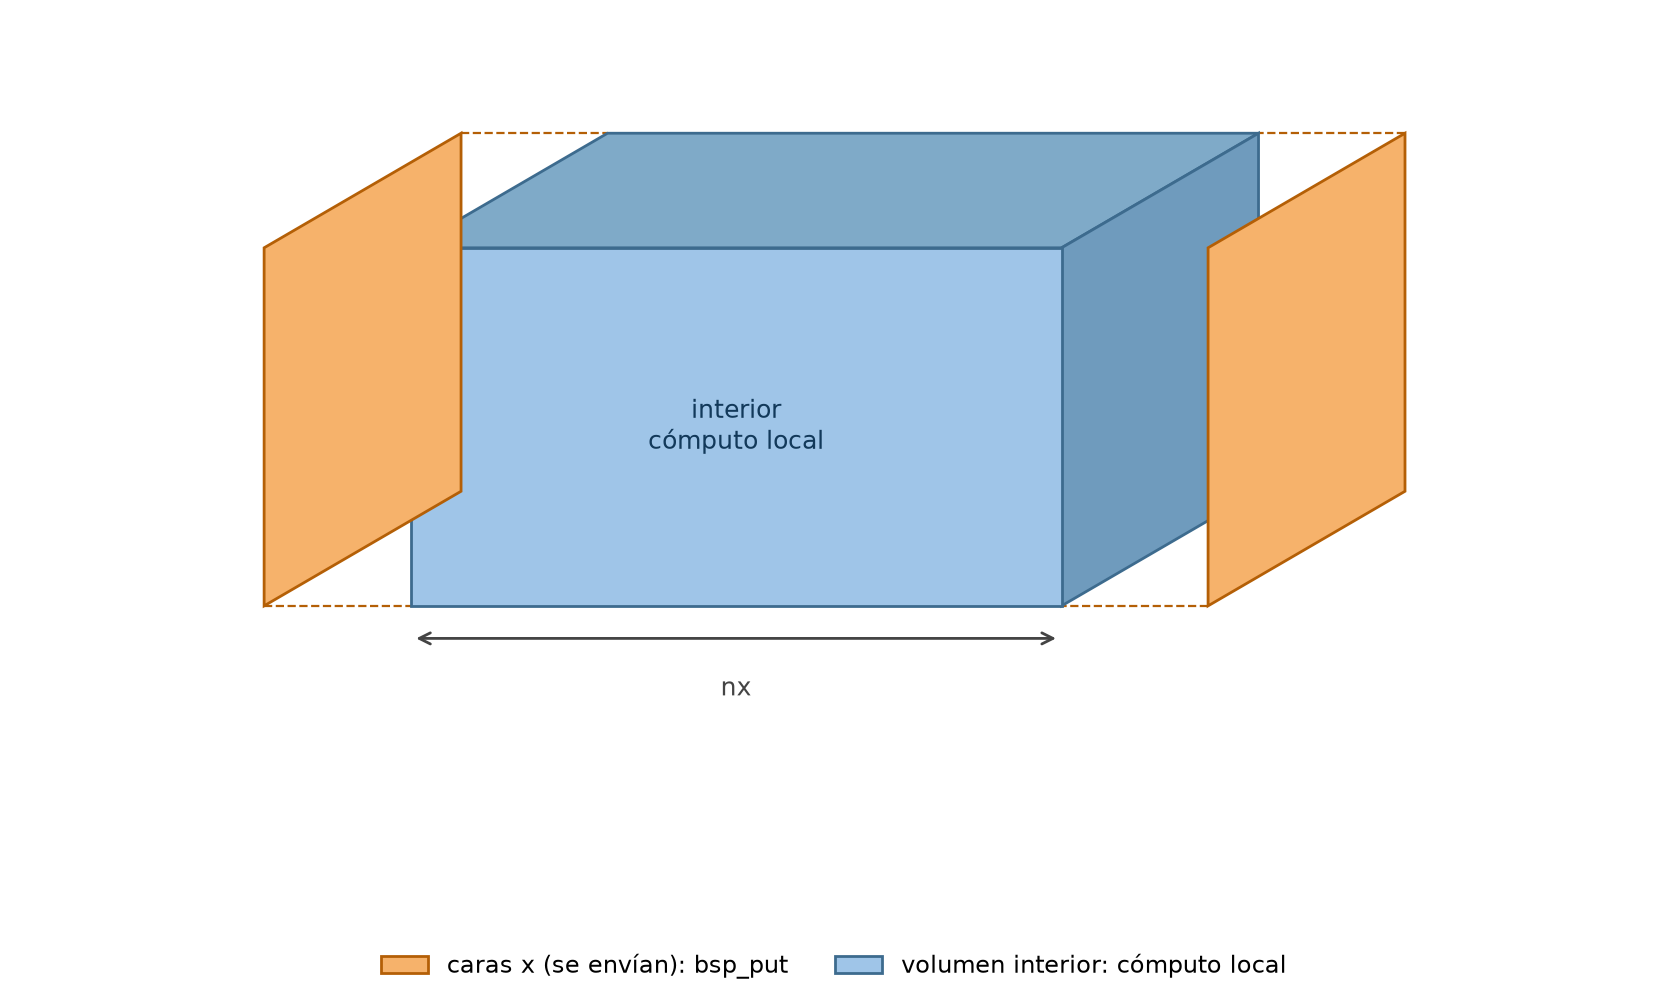
\includegraphics[width=0.78\textwidth]{communication_volume_3d.png}\par
  \vspace{-2mm}
  {\scriptsize Las caras naranjas se envían; el volumen azul se calcula
   localmente.}
\end{frame}

\begin{frame}{Detalle del intercambio de halos}
  \centering
  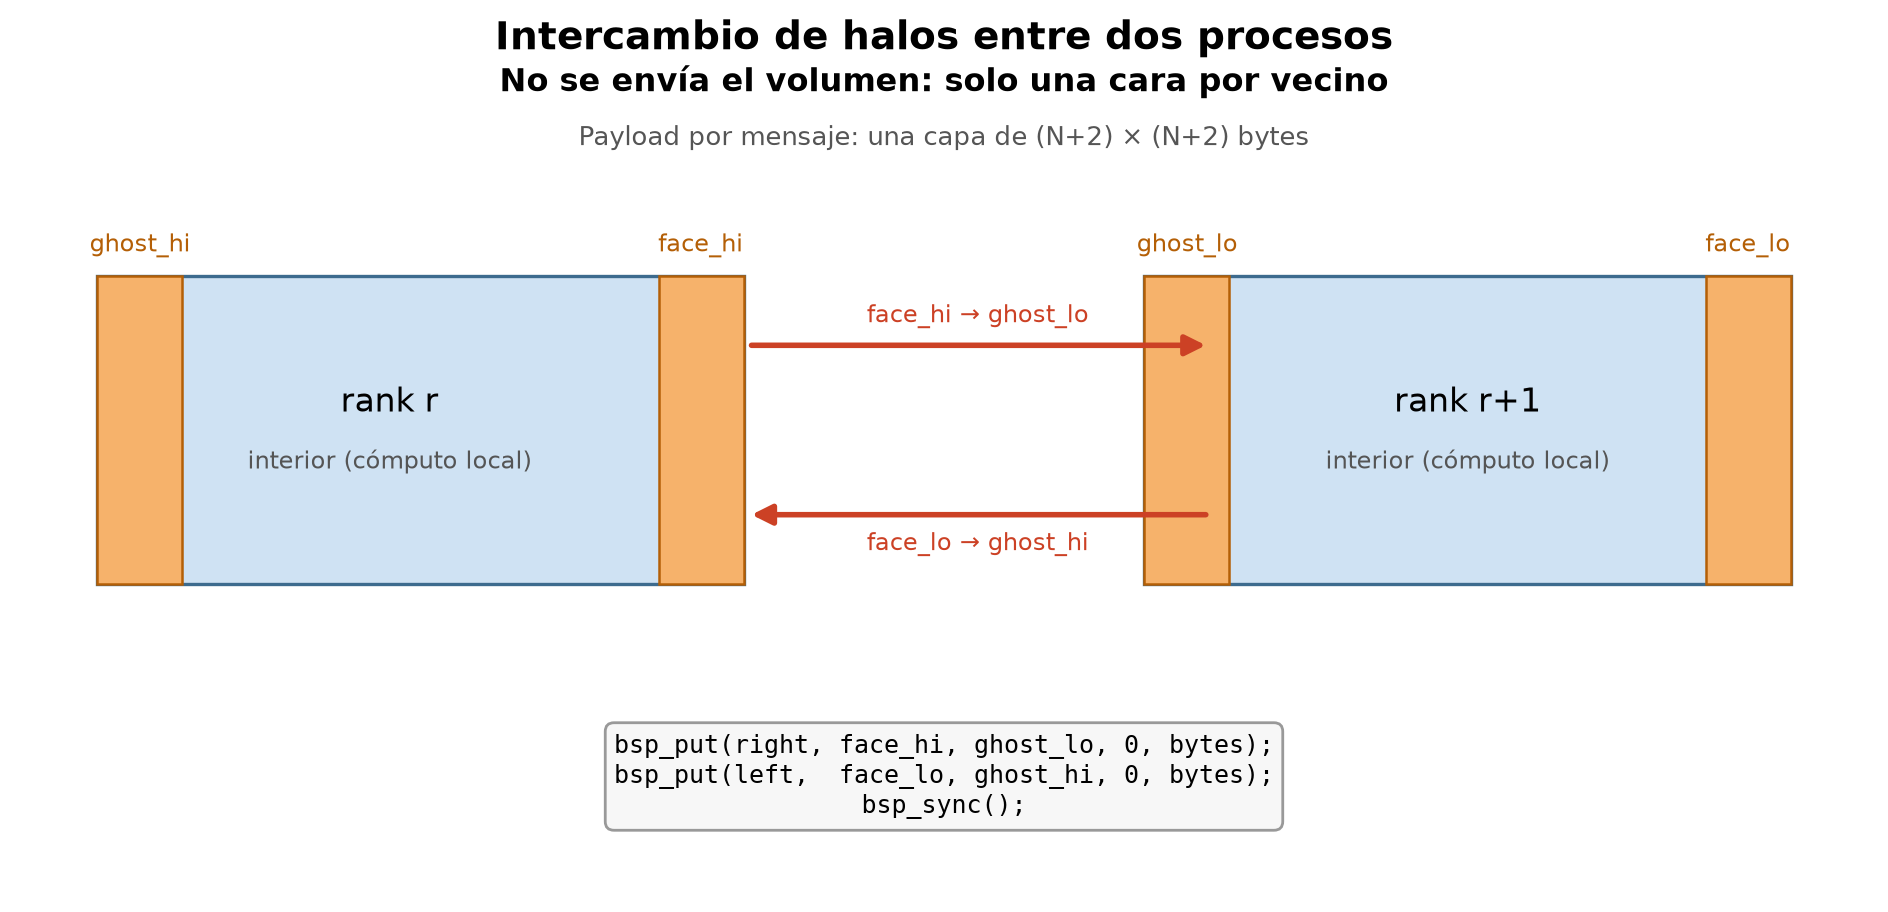
\includegraphics[width=0.95\textwidth]{halo_exchange.png}\par
  \vspace{-1mm}
  {\scriptsize \texttt{bsp\_put} escribe en el ghost del vecino;
   \texttt{bsp\_sync} hace visible la comunicación diferida.}
\end{frame}

\begin{frame}{Procesos e hilos}
  \centering
  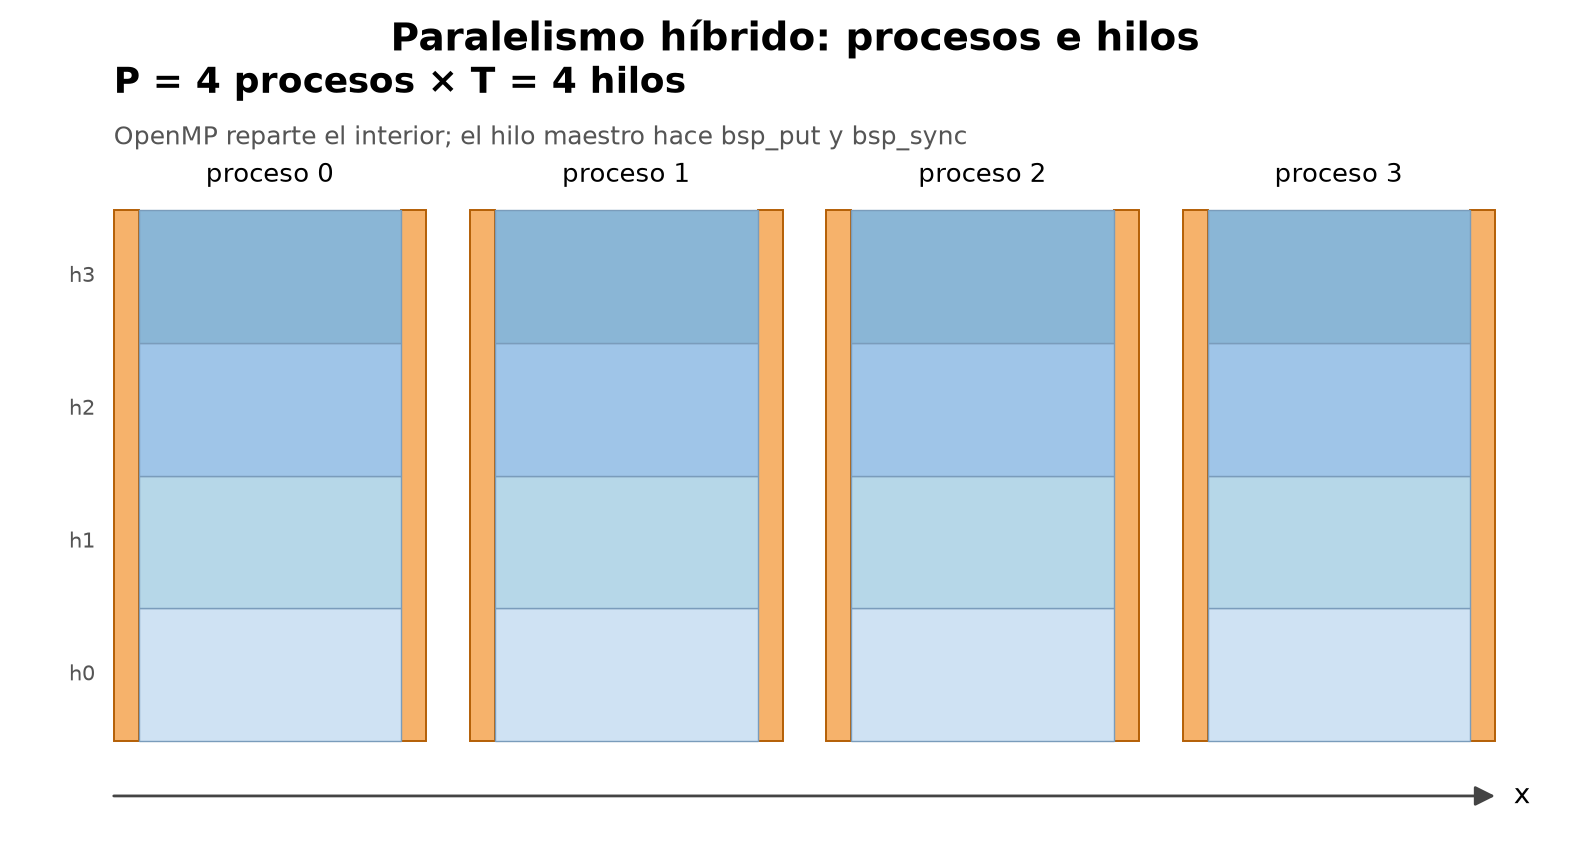
\includegraphics[width=0.80\textwidth]{hybrid_threads.png}\par
  \vspace{-1mm}
  {\scriptsize $P=4$ procesos, $T=4$ hilos; OpenMP reparte el interior y el
   hilo maestro se encarga de la comunicación.}
\end{frame}

\begin{frame}[fragile]{Hilos y thread safety}
  \begin{columns}[T]
    \begin{column}{0.55\textwidth}
      \begin{itemize}
        \item OpenMP en colisión, streaming, métricas y densidad.
        \item \texttt{collapse(3)} sobre $(x,y,z)$.
        \item BSPlib \alert{no} es thread-safe.
        \item Llamadas BSPlib solo desde el hilo maestro, fuera de las
              regiones paralelas.
        \item Una región OpenMP por fase, con barrera implícita.
      \end{itemize}
      \begin{block}{Decisión}
        \footnotesize
        Evita condiciones de carrera y mantiene el modelo BSP: cómputo
        paralelo, comunicación serial, \texttt{bsp\_sync}.
      \end{block}
    \end{column}
    \begin{column}{0.43\textwidth}
      \begin{lstlisting}[language=C++,basicstyle=\ttfamily\tiny,
                         breaklines=true,frame=single]
#pragma omp parallel for collapse(3)
for (x...) for (y...) for (z...)
    collide_or_stream(x,y,z);

bsp_put(left,  lo, ghost_hi, 0, bytes);
bsp_put(right, hi, ghost_lo, 0, bytes);
bsp_sync();
      \end{lstlisting}
    \end{column}
  \end{columns}
\end{frame}

\begin{frame}[fragile]{Implementación: stack y build}
  \begin{itemize}
    \item C++17, OpenMP, OpenMPI 4.1.6, BSPonMPI 0.3.
    \item \texttt{src/gas.cpp}: autómata + driver BSP/OpenMP + VTK.
    \item \texttt{CMakeLists.txt}, \texttt{docker/Dockerfile},
          \texttt{scripts/}.
    \item Compilar con \texttt{-DOMPI\_SKIP\_MPICXX} (OpenMPI 4.x).
  \end{itemize}
  \vspace{1mm}
  \begin{lstlisting}[language=bash,basicstyle=\ttfamily\scriptsize,
                     breaklines=true,frame=single]
docker build -t hpc-lab2:latest -f docker/Dockerfile .
./scripts/docker_shell.sh bash -lc './scripts/build.sh'
GEOM=chamber P_RATIO=10 RAMP=8 OMP_NUM_THREADS=4 \
  mpirun -np 4 --bind-to none ./build/gas 256 1000 4 100 chamber
  \end{lstlisting}
\end{frame}

% ---------------------------------------------------------------------------
\section{Validación y plan de experimentos}
% ---------------------------------------------------------------------------

\begin{frame}{Plan de validación}
  \centering
  \scriptsize
  \begin{tabular}{>{\raggedright\arraybackslash}p{3.2cm}>{\raggedright\arraybackslash}p{5.0cm}>{\raggedright\arraybackslash}p{4.8cm}}
    \toprule
    Criterio & Prueba & Éxito \\
    \midrule
    Masa y momento & Suma global antes y después de cada corrida &
    Iguales exactamente \\
    Halos & Test sintético de intercambio en 4 ranks &
    0 errores \\
    Serial vs.\ paralelo & Misma malla y pasos, $P=1$ vs.\ $P=4$, comparar
    \texttt{.vti} & Idénticos byte a byte \\
    Salida & Suma de densidad del VTK vs.\ masa global &
    Coinciden \\
    Híbrido & 4 procesos $\times$ 4 hilos & Todos los ranks reportan 4 hilos \\
    Rendimiento & Matriz $P\times T$ & Speedup y eficiencia medidos \\
    \bottomrule
  \end{tabular}
  \vspace{3mm}
  \begin{block}{Criterio de aceptación}
    \footnotesize
    Si falla la conservación o la comparación byte a byte, se revisa primero
    la tabla de colisión y luego el mapeo de halos. No se aceptan resultados
    de \emph{scaling} sin validación previa.
  \end{block}
\end{frame}

\begin{frame}{Plan de experimentos}
  \begin{columns}[T]
    \begin{column}{0.50\textwidth}
      \begin{block}{Configuraciones}
        \scriptsize
        \begin{tabular}{ll}
          \toprule
          Config & Objetivo \\
          \midrule
          $1\times1$ & baseline serial \\
          $1\times T$ & escalado OpenMP \\
          $P\times1$ & escalado de procesos \\
          $P\times T$ & híbrido \\
          $4\times8$ & objetivo en nodo de 32 hilos \\
          \bottomrule
        \end{tabular}
      \end{block}
    \end{column}
    \begin{column}{0.48\textwidth}
      \begin{block}{Parámetros}
        \scriptsize
        \begin{itemize}
          \item $N=128,256,512$; pasos fijos.
          \item 3 repeticiones, mediana.
          \item Sin VTK para medir; \texttt{--bind-to none}.
          \item Métricas: tiempo de loop, cómputo, comunicación.
          \item \emph{Strong} y \emph{weak scaling}.
        \end{itemize}
      \end{block}
    \end{column}
  \end{columns}
  \vspace{2mm}
  \begin{block}{Hipótesis a verificar (no resultados)}
    \footnotesize
    El problema es \emph{memory-bound}: OpenMP escalará hasta saturar los
    núcleos físicos; los procesos no mejorarán el tiempo en un solo nodo por
    el costo de \texttt{bsp\_sync}; en varios nodos sí serán necesarios.
  \end{block}
\end{frame}

% ---------------------------------------------------------------------------
\section{Riesgos y decisiones}
% ---------------------------------------------------------------------------

\begin{frame}{Riesgos y mitigación}
  \centering
  \scriptsize
  \begin{tabular}{>{\raggedright\arraybackslash}p{4.2cm}>{\raggedright\arraybackslash}p{9.0cm}}
    \toprule
    Riesgo & Mitigación \\
    \midrule
    BSPonMPI 0.3 antiguo (SCons/Python 2) &
    Compilar a mano; fijar versión; Docker reproducible \\
    \texttt{bsp\_get\_tag} incluye el tag &
    Restar \texttt{sizeof(int)} antes de \texttt{bsp\_move}; documentado \\
    BSPlib no thread-safe &
    Llamadas solo desde el hilo maestro; comunicación serial \\
    Costo de comunicación con $P$ grande &
    Medir fracción de comunicación; elegir $P$ según el tamaño local \\
    No hay nodo de 32 hilos &
    Correr $4\times4$ local y $4\times8$ en el cluster; reportar ambos \\
    Modelo isotérmico &
    Declararlo; LGA térmico como trabajo futuro \\
    Anisotropía del LGA &
    Comparar tendencias cualitativas; evaluar partícula en reposo \\
    Bordes periódicos &
    Declararlo; paredes reflectantes como opción futura \\
    \bottomrule
  \end{tabular}
\end{frame}

\begin{frame}{Alternativas consideradas}
  \centering
  \scriptsize
  \begin{tabular}{>{\raggedright\arraybackslash}p{3.2cm}>{\raggedright\arraybackslash}p{3.6cm}>{\raggedright\arraybackslash}p{6.2cm}}
    \toprule
    Decisión & Alternativa & Por qué se eligió \\
    \midrule
    LGA 6 direcciones & LBM / stencil PDE &
    Requisito de autómata celular; estado entero y conservación exacta \\
    BSPlib + OpenMP & MPI + OpenMP directo &
    Requisito de BSP; superpasos y comunicación por bloques \\
    Descomposición 1D & 2D / 3D &
    Solo 2 vecinos, implementación simple; 2D/3D como mejora \\
    Bordes periódicos & Paredes reflectantes &
    Adecuado para \emph{scaling}; paredes para un recipiente cerrado \\
    Cámara 10:1 & Solo esfera &
    Gradiente de presión explícito y razón finita; esfera como baseline \\
    Neón & Helio &
    $c_s$ moderada y densidad fácil de verificar; He como alternativa \\
    VTK + CSV & Solo VTK &
    VTK para 3D; CSV para evolución temporal y métricas \\
    \bottomrule
  \end{tabular}
\end{frame}

\begin{frame}{Resumen de decisiones}
  \begin{itemize}
    \item \alert{Modelo}: LGA 3D de 6 direcciones, sin reposo, con exclusión.
    \item \alert{Física}: gas ideal monoatómico (neón), con corrección del
          virial despreciable y limitación isotérmica declarada.
    \item \alert{Geometría}: esfera base + cámara 10:1 con gradiente
          controlado.
    \item \alert{Paralelización}: BSP/BSPlib para procesos, OpenMP para hilos,
          descomposición 1D y halos con \texttt{bsp\_put}.
    \item \alert{Validación}: invariantes exactos, test de halos y comparación
          $P=1$ vs.\ $P=4$ byte a byte.
    \item \alert{Experimentos}: matriz $P\times T$, strong/weak scaling y
          fracción de comunicación; $4\times8$ en nodo de 32 hilos.
  \end{itemize}
\end{frame}

\begin{frame}{Preguntas para la discusión}
  \begin{enumerate}
    \item ¿El LGA de 6 direcciones es aceptable como autómata celular para el
          curso, o se prefiere un modelo con partícula en reposo?
    \item ¿La cámara 10:1 es la geometría adecuada, o conviene una esfera con
          fondo de baja presión?
    \item ¿Se exige una expansión adiabática? Si es así, hay que cambiar a un
          modelo térmico.
    \item ¿Habrá acceso a un nodo de 32 hilos para el $4\times8$?
    \item ¿Se prefieren paredes reflectantes o periódicas?
  \end{enumerate}
\end{frame}

\begin{frame}
  \centering
  \Huge Gracias\\[4mm]
  \normalsize ¿Preguntas?
\end{frame}

\end{document}
